\chapter{Societal Contribution, Deployment Program, and the Next Parity Frontier}
\label{ch:societal-roadmap}

The strongest societal contribution of ORIUS is not that it solves every safety problem
in physical AI.  It is that it names a failure mode that repeatedly appears across
domains and turns that failure mode into a runtime object that can be monitored,
repaired, certified, and audited.  If that contribution holds, ORIUS becomes useful far
beyond a single battery benchmark.

The deployment story follows the parity gate, not aspiration alone. The next frontier is not a new slogan; it is closing navigation with real-data evidence, replacing the aerospace placeholder with a real multi-flight safety task, and expanding cross-domain runtime governance and composition only where the same governed artifacts actually clear.
That is how ORIUS can contribute meaningfully to society without borrowing credibility
from unclosed rows.

\section{Runtime breadth and governance maturity}
The 93+ program also makes runtime breadth explicit.  The point is not simply that
CertOS exists; it is that runtime budgets, lifecycle events, and audit continuity are
now tabled across the defended rows rather than treated as battery-only depth.

\begin{table*}[htbp]
\centering
\scriptsize
\caption{Cross-domain runtime-budget matrix for the ORIUS 93+ closure program. Battery uses the locked witness latency surface; the remaining rows use the SIL summary and domain-closure runtime traces.}
\label{tab:orius-runtime-budget-matrix}
\resizebox{\textwidth}{!}{%
\begin{tabular}{p{2.3cm}p{2.3cm}p{2.3cm}p{2.3cm}p{2.3cm}p{2.3cm}p{2.3cm}p{2.3cm}p{2.3cm}p{2.3cm}}
\toprule
\textbf{Domain} & \textbf{P95 step latency (ms)} & \textbf{Mean reliability} & \textbf{Repair rate (\%)} & \textbf{Certificate rate (\%)} & \textbf{Runtime error (\%)} & \textbf{Fallback mode} & \textbf{CertOS} & \textbf{Runtime depth} & \textbf{Exact limit}\\
\midrule
Battery Energy Storage & 0.1193 & witness\_reference & n/a\_reference & 100.0 & 0.0 & safe\_hold & evaluated & reference\_runtime & external bench and field telemetry packaging still remain bounded deployment items\\
Autonomous Vehicles & 0.255 & 0.682 & 100.0 & 100.0 & 0.0 & full\_brake & evaluated & proof\_validated & multi\_lane\_and\_higher\_dimensional\_repair\_open\\
Industrial Process Control & 0.579 & 0.575 & 83.3 & 100.0 & 0.0 & power\_cap & evaluated & proof\_validated & bounded\_to\_current\_plant\_family\\
Medical and Healthcare Monitoring & 0.763 & 0.731 & 20.8 & 100.0 & 0.0 & max\_alert & evaluated & proof\_validated & bounded\_to\_current\_monitoring\_and\_intervention\_contract\\
Navigation and Guidance & 0.864 & 0.799 & 100.0 & 100.0 & 0.0 & hold\_position & gated & shadow\_synthetic & navigation\_real\_data\_row\_missing\\
Aerospace Control & 0.454 & 0.707 & 25.0 & 100.0 & 0.0 & envelope\_hold & gated & experimental & real\_multi\_flight\_safety\_task\_missing\\
\bottomrule
\end{tabular}}
\end{table*}


\begin{table}[htbp]
\centering
\caption{Governance lifecycle matrix for the active Battery + AV + Healthcare program.}
\label{tbl:orius-governance-lifecycle-matrix}
\begin{tabular}{lllll}
\toprule
Domain & Tier & Governance Surface & Lifecycle State & Note\\
\midrule
Battery Energy Storage & reference & certified\_runtime & witness\_locked & Battery remains the deepest certificate and theorem witness row.\\
Autonomous Vehicles & proof\_validated & certified\_runtime & bounded\_promoted & AV is promoted only under the TTC plus predictive-entry-barrier contract.\\
Medical and Healthcare Monitoring & proof\_validated & certified\_runtime\_proxy & bounded\_promoted & Healthcare remains bounded to monitoring and alert semantics with explicit governance-proxy wording.\\
\bottomrule
\end{tabular}
\end{table}


\begin{figure}[htbp]
\centering
\IfFileExists{reports/publication/fig_orius_runtime_governance_matrix.png}{%
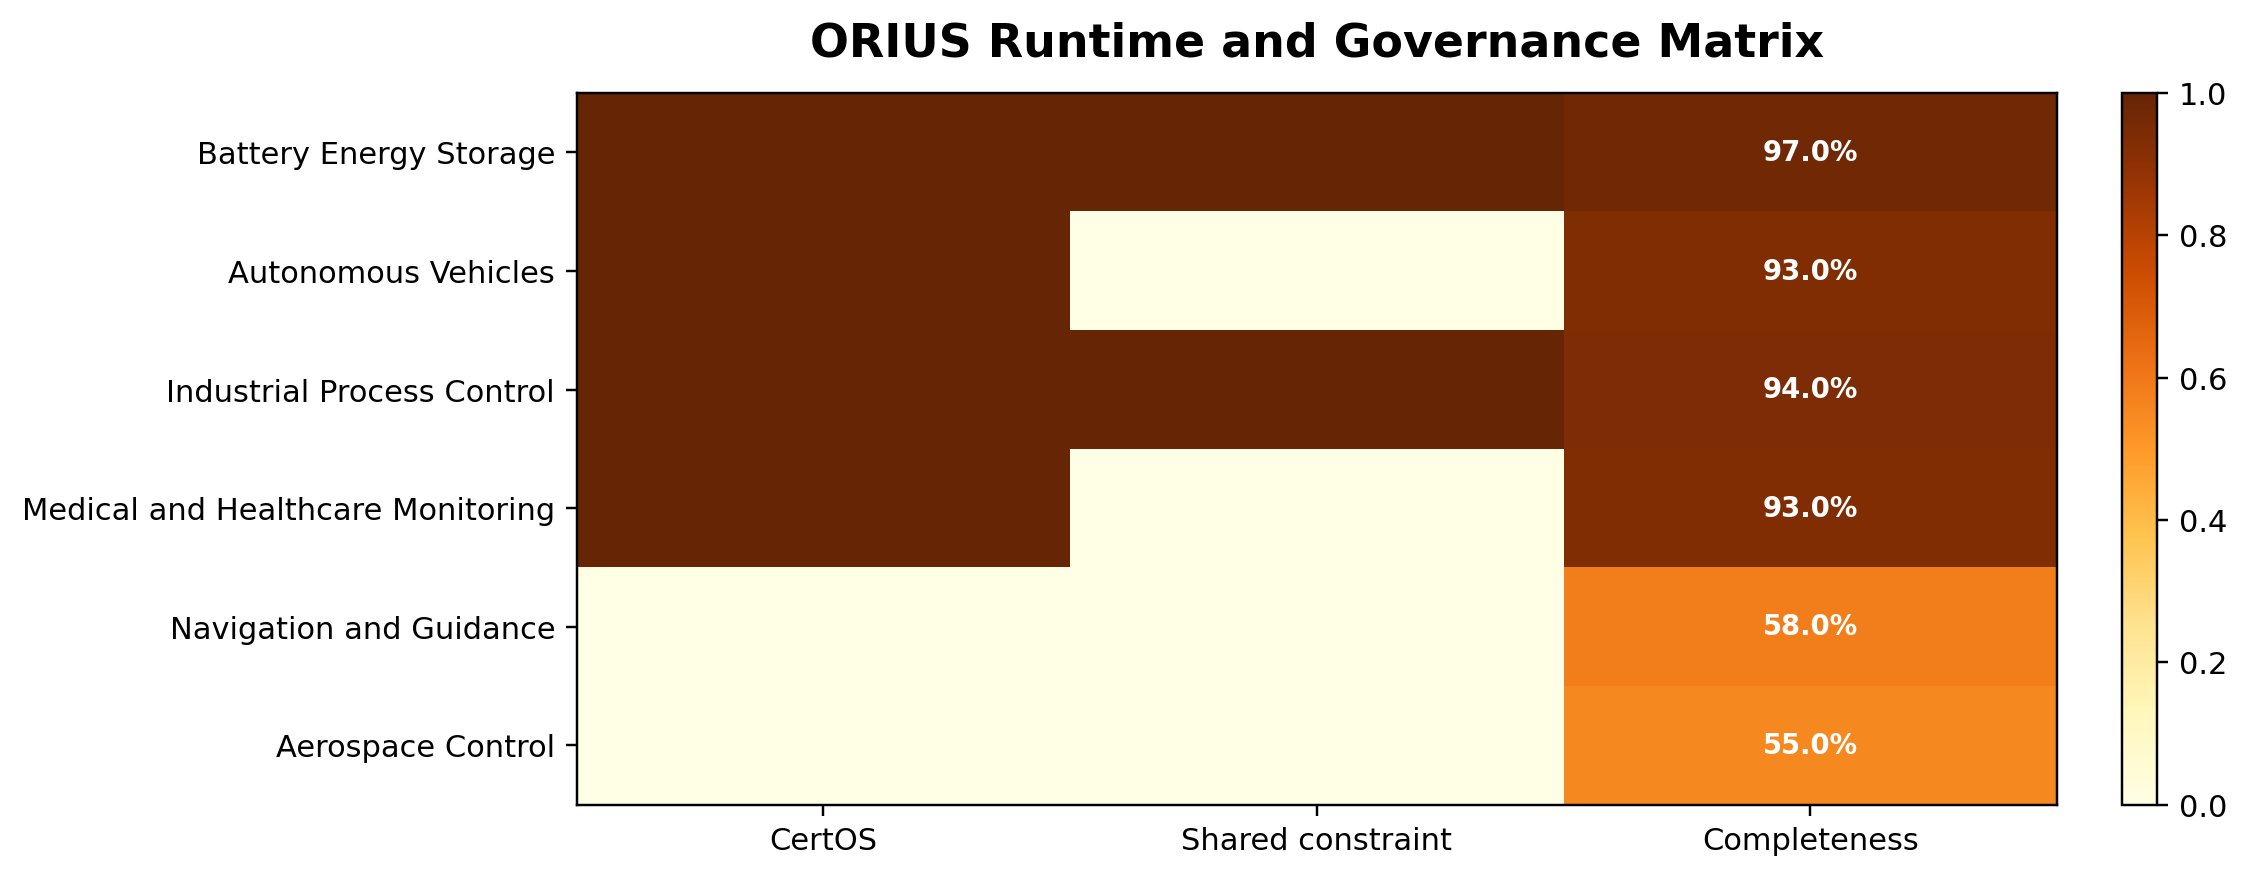
\includegraphics[width=0.88\textwidth]{reports/publication/fig_orius_runtime_governance_matrix.png}%
}{%
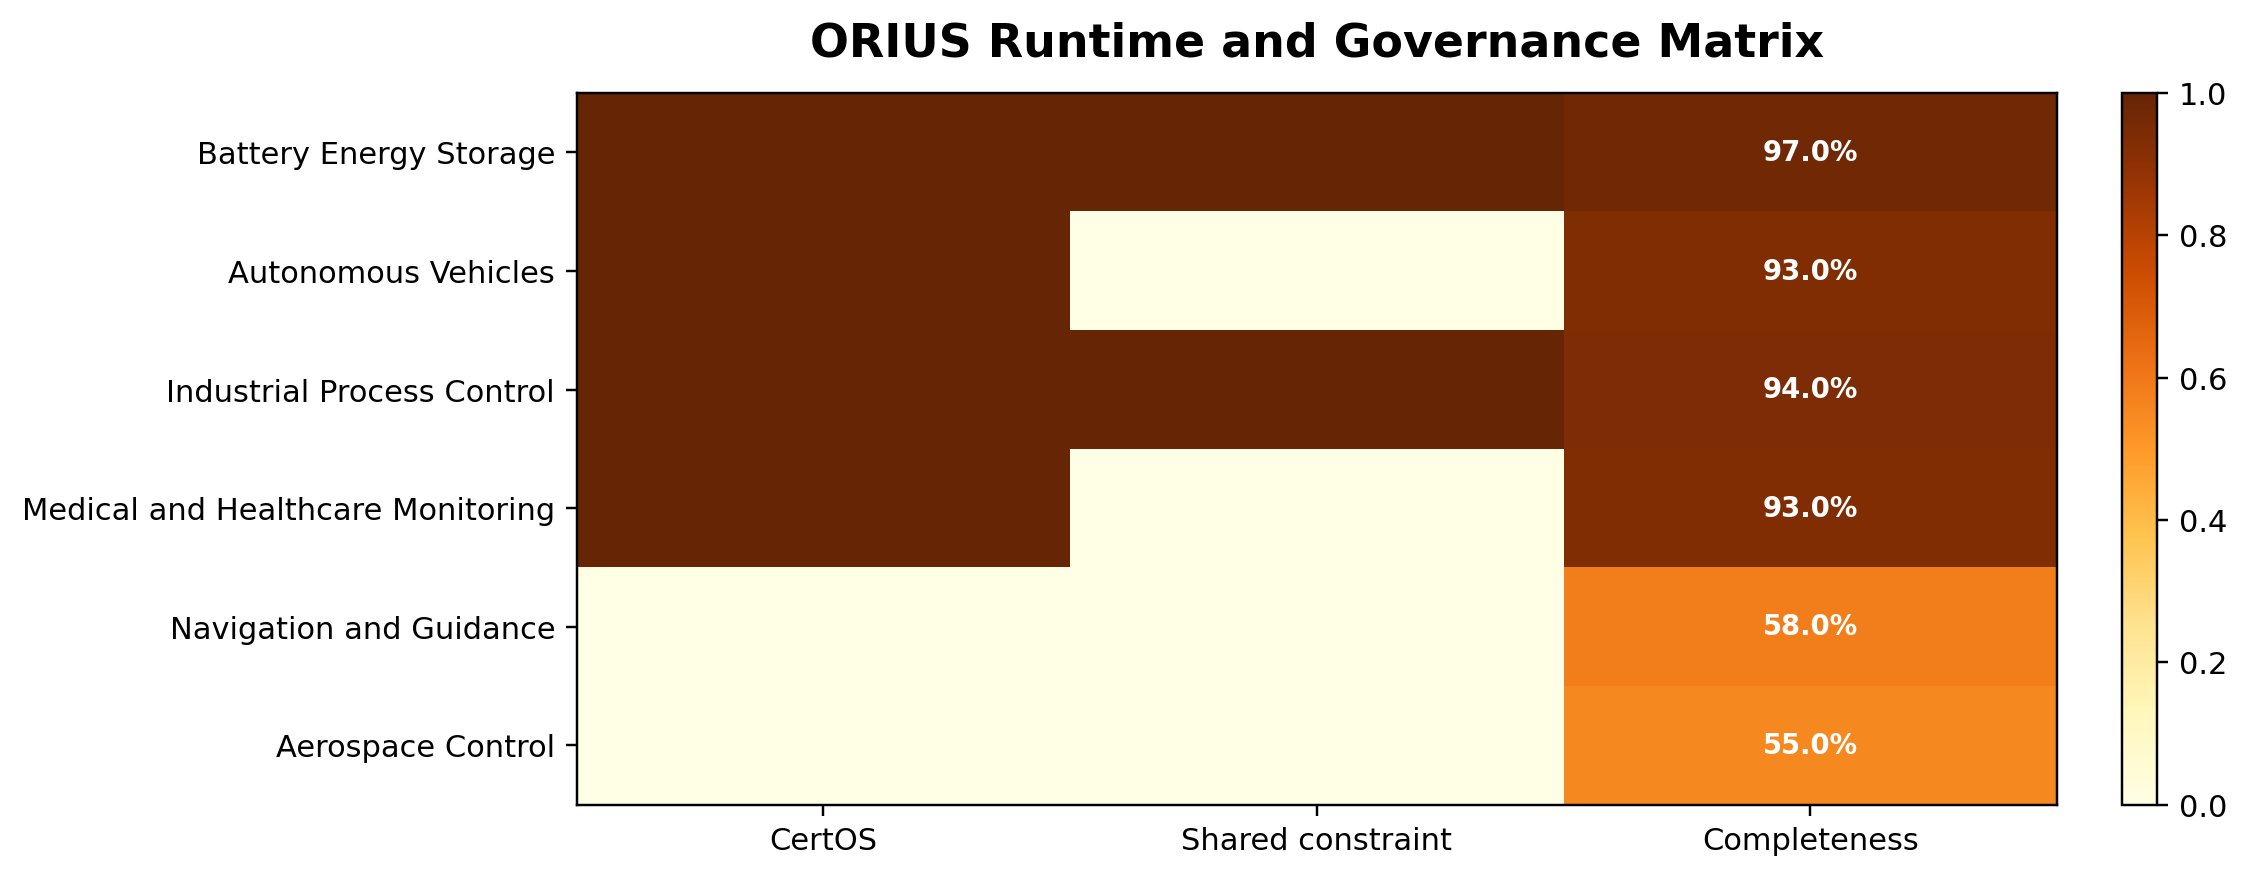
\includegraphics[width=0.88\textwidth]{../reports/publication/fig_orius_runtime_governance_matrix.png}%
}
\caption{Cross-domain runtime and governance matrix showing CertOS lifecycle coverage, shared-constraint evaluation, and governance completeness.}
\label{fig:orius-runtime-governance-matrix}
\end{figure}

\section{Deployment validation scope}
ORIUS should only use deployment language that matches the evidence surface.  The
deployment-scope table below distinguishes defended replay, HIL rehearsal, proxy
validation, and explicitly open field or regulated surfaces.  This keeps the societal
pitch strong without letting aspiration flatten the current evidence hierarchy.

\begin{table}[htbp]
\centering
\caption{Deployment validation scope for the active Battery + AV + Healthcare program.}
\label{tbl:orius-deployment-validation-scope}
\begin{tabular}{llllll}
\toprule
Deployment Surface & Governing Artifact & Scope Type & Current Status & Bounded Claim & Exact Non-Claim or Gap\\
\midrule
Battery runtime and HIL rehearsal & reports/publication/dc3s\_latency\_summary.csv; reports/hil/hil\_summary.json & rehearsal\_plus\_hil & bounded\_reference & Battery supports the deepest runtime and HIL-backed evidence in the defended program. & This is still not a full external bench or unrestricted field deployment package.\\
Battery aging and half-life & reports/aging/asset\_preservation\_proxy\_table.csv; reports/publication/aging\_aware\_calibration\_design.md & proxy\_plus\_design & partial & The monograph can defend proxy-backed aging and half-life design reasoning. & It does not yet defend a full live aging-validation stack.\\
Autonomous-vehicle defended replay & reports/orius\_av/nuplan\_allzip\_grouped\_runtime\_dropout\_aligned\_m15\_fulltest/runtime\_summary.csv & bounded\_replay & defended\_bounded & AV supports bounded nuPlan replay under the runtime contract. & It does not claim full autonomous-driving field closure or live road deployment.\\
Healthcare defended replay & reports/healthcare/runtime\_summary.csv; reports/healthcare/runtime\_governance\_summary.csv; data/healthcare/mimic3/processed/mimic3\_manifest.json & bounded\_replay & defended\_bounded & Healthcare supports bounded monitoring and alert-release claims on the canonical MIMIC row. & It does not claim regulated clinical deployment or a stronger clinical-release theorem beyond the bounded replay row.\\
OOD and adversarial completeness & chapters/ch34\_outside\_current\_evidence.tex; reports/publication/adversarial\_probing\_robustness\_table.csv & explicit\_non\_claim\_register & bounded\_non\_claim & The monograph can discuss bounded active probing and non-claim discipline. & It does not claim universal adversarial completeness or unrestricted OOD safety.\\
\bottomrule
\end{tabular}
\end{table}

